\documentclass[12pt, a4paper]{report}
\usepackage{graphicx, array, amsthm, amssymb, amsmath, algorithm, algpseudocode, float, xcolor, thmtools, thmbox, chronology}
\usepackage[english]{babel}

\makeatletter
\renewcommand\thmbox@headstyle[2]{\bfseries #1}
\makeatother
\newtheorem[style=M,bodystyle=\normalfont]{theorem}{Theorem}
\newtheorem[style=M,bodystyle=\normalfont]{corollary}{Corollary}
\newtheorem[style=M,bodystyle=\normalfont]{lemma}{Lemma}
\newtheorem[style=M,bodystyle=\normalfont]{definition}{Definition}


\title{Data Bases II \\ \textit{Theory}}
\author{Christian Rossi}
\date{Academic Year 2023-2024}

\begin{document}

\maketitle

\newpage

\begin{abstract}
    The course aims to prepare software designers on the effective development of database applications. First, the course presents the fundamental features of current database 
    architectures, with a specific emphasis on the concept of transaction and its realization in centralized and distributed systems. Then, the course illustrates the main directions 
    in the evolution of database systems, presenting approaches that go beyond the relational model, like active databases, object systems and XML data management solutions.
\end{abstract}

\newpage

\tableofcontents

\newpage

\chapter{Introduction}
    \section{Data Base Management System}
    \begin{definition}
        A \emph{Data Base Management System} is a software product capable of managing data collections that are: 
        \begin{itemize}
            \item Large: much larger than the central memory available on the computers that run the software. 
            \item Persistent: with a lifetime which is independent of single executions of the programs that access them. 
            \item Shared: used by several applications at a time. 
            \item Reliable: ensuring tolerance to hardware and software failures. 
            \item Data ownership respectful: by disciplining and controlling accesses. 
        \end{itemize}
    \end{definition}
    \begin{chronology}[5]{1990}{2020}{\textwidth}
        \event{1992}{SQL '92}
        \event{1999}{SQL '99}
        \event{2001}{ranking in databases}
        \event{2003}{XML-related features}
        \event{2005}{NoSQL}
        \event{2006}{X-Query}
        \event{2009}{JPA final release}
        \event{2011}{Temporal databases}
        \event{2016}{JSON}
    \end{chronology}

    \section{Transactions}
    \begin{definition}
        A \emph{transaction} is an elementary, atomic unit of work performed by an application. Each transaction is conceptually encapsulated within two commands:
        \begin{itemize}
            \item Begin transaction.
            \item End transaction.
        \end{itemize}
    \end{definition}
    Within a transaction, one of the commands below is executed to signal the end of the transaction:
    \begin{itemize}
        \item Commit-work (commit). 
        \item Rollback-work (abort). 
    \end{itemize}
    \begin{definition}
        The \emph{On-Line Transaction Processing} (OLTP) is a system that supports the execution of transactions on behalf of concurrent applications. 
    \end{definition}
    The application can run many transactions. So, the transactions are part of the application and not vice-versa. The transactions follow the ACID property: 
    \begin{enumerate}
        \item Atomicity: a transaction is an indivisible unit of execution. This means that all the operations in the transaction are executed or none is executed. The time in which 
            commit is executed marks the instant in which the transaction ends successfully: an error before should cause the rollback and an error after should not alter the transaction.
            The rollback of the work performed can be caused by a rollback statement or by the DBMS. In case of a rollback, the work performed must be undone, bringing the database to 
            the state it had before the start of the transaction. It is the application's responsibility to decide whether an aborted transaction must be redone or not. 
        \item Consistency: A transaction must satisfy the database integrity constraints: if the initial state $S_0$ is consistent, then the final state $S_f$ is also consistent. 
            This is not necessarily true for the intermediate states $S_i$. For example, the sum of the worked hours per task should equal the planned work hours of the project. 
            If the constraint holds before the transaction it must hold also after its execution. The constraint can be temporarily violated during the execution of the transaction 
            (e.g., when shifting work from a task tom another one, but must be satisfied at the end). 
        \item Isolation: the execution of a transaction must be independent of the concurrent execution of other transactions. In particular, the concurrent execution of a number 
            of transactions must produce the same result as the execution of the same transactions in a sequence. Isolation impacts performance and trade-offs can be defined between 
            isolation and performance. 
        \item Durability: The effect of a transaction that has successfully committed will last forever, independently of any system fault. 
    \end{enumerate}
    \begin{table}[H]
        \centering
        \begin{tabular}{c|c|l}
        \textbf{Property} & \textbf{Actions}       & \textbf{Architectural element} \\ \hline
        Atomicity         & Abort-rollback-restart & Query Manager                  \\
        Consistency       & Integrity checking     & Integrity Control System       \\
        Isolation         & Concurrency control    & Concurrency Control System     \\
        Durability        & Recovery management    & Reliability Manager           
        \end{tabular}
    \end{table}
    \begin{figure}[H]
        \centering
        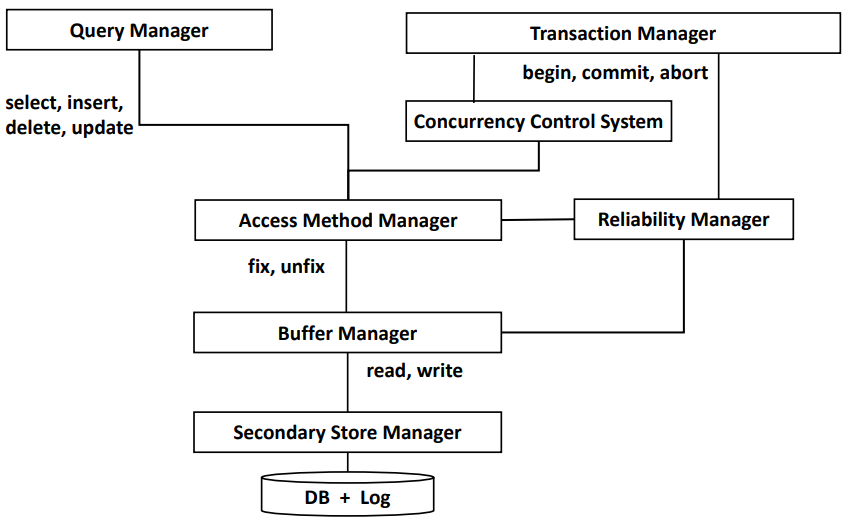
\includegraphics[width=0.75\linewidth]{images/architecture.png}
        \caption{Architecture of a Data Base Management System}
    \end{figure}

\newpage

\chapter{Concurrency}
    \section{Introduction}
    A DBMS usually needs to manage multiple applications. A unit of measurement used to evaluate the DBMS workload is the number of transaction per second (tps) handled by it. 
    To have an efficient usage of the database the DBMS needs to be able to handle concurrency while avoiding the insurgence of anomalies. 
    The concurrency control system schedules the order of the various transactions. 
    
    \section{Anomalies in concurrent transactions}
    The typical types on anomalies in concurrency are: 
    \begin{itemize}
        \item Lost update: an update is applied from a state that ignores a preceding update, which is lost.
            \begin{table}[H]
                \centering
                \begin{tabular}{c|c}
                \textbf{Transaction $t_1$}    & \textbf{Transaction $t_2$} \\ \hline
                $r_1(x)$                      &                            \\
                $x=x+1$                       &                            \\
                                              & $r_2(x)$                   \\
                                              & $x=x+1$                    \\
                                              & $w_2(x)$                   \\
                                              & commit                     \\
                $w_1(x)$                      &                            \\
                commit                        &                           
                \end{tabular}
            \end{table}
        \item Dirty read: an uncommitted value is used to update the data. 
            \begin{table}[H]
                \centering
                \begin{tabular}{c|c}
                \textbf{Transaction $t_1$} & \textbf{Transaction $t_2$} \\ \hline
                $r_1(x)$                   &                            \\
                $x=x+1$                    &                            \\
                $w_1(x)$                   &                            \\
                                        & $r_2(x)$                   \\
                                        & commit                     \\
                abort                      &                           
                \end{tabular}
            \end{table}
        \item Non-repeatable read: someone else updates a previously read value.
            \begin{table}[H]
                \centering
                \begin{tabular}{c|c}
                \textbf{Transaction $t_1$}  & \textbf{Transaction $t_2$} \\ \hline
                $r_1(x)$                    &                            \\
                                            & $r_2(x)$                   \\
                                            & $x=x+1$                    \\
                                            & $w_2(x)$                   \\
                                            & commit                     \\
                $r_1(x)$                    &                            \\
                commit                      & \multicolumn{1}{l}{}      
                \end{tabular}
            \end{table}
        \item Phantom update: someone else updates data that contributes to a previously valid constraint. 
            \begin{table}[H]
                \centering
                \begin{tabular}{c|c}
                \textbf{Transaction $t_1$} & \textbf{Transaction $t_2$} \\ \hline
                $r_1(x)$                   &                            \\
                                           & $r_2(y)$                   \\
                $r_1(y)$                   &                            \\
                                           & $y=y-100$                  \\
                                           & $r_2(z)$                   \\
                                           & $z=z+100$                  \\
                                           & $w_2(y)$                   \\
                                           & $w_2(z)$                   \\
                                           & commit                     \\
                $r_1(z)$                   &                            \\
                $s=x+y+z$                  &                            \\
                commit                     &                           
                \end{tabular}
            \end{table}
        \item Phantom insert: someone else inserts data that contributes to a previously read datum.
    \end{itemize}

    \section{Concurrency theory}
    \begin{definition}
        A \emph{model} is an abstraction of a system, object or process, which purposely disregards details to simplify the investigation of relevant properties. 
    \end{definition}
    Concurrency theory builds upon a model of transaction and concurrency control principles that help understanding the real systems. Real systems exploit implementation level 
    mechanisms (locks, snapshots) which help achieve some desirable properties postulated by the theory. 
    \begin{definition}
        An \emph{operation} consist in a reading or in a writing of a specific datum by a specific transaction. 
    \end{definition}
    \begin{definition}
        A \emph{schedule} is a sequence of operations performed by concurrent transactions that respects the order of operations of each transaction. 
    \end{definition}
    The transactions can be: serial, interleaved or nested. The number of serial schedules for $n$ transaction is equal to 
    \[N_S=n!\]
    while the total number of distinct schedules given the number of transaction $n$ is equal to: 
    \[N_D=\dfrac{\left( \sum_{i=1}^nk_i \right)!}{\prod_{i=1}^n \left( k_i! \right)}\]
    \begin{example}
        Given two transaction $T_1$ and $T_2$ we have six possible different schedules, where only two are serial:
        \begin{enumerate}
            \item $r_1(x) \rightarrow w_1(x) \rightarrow r_2(z) \rightarrow w2(z)$
            \item $r_2(z) \rightarrow w_2(z) \rightarrow r_1(x) \rightarrow w_1(x)$
            \item $r_1(x) \rightarrow r_2(z) \rightarrow w_1(x) \rightarrow w_2(z)$
            \item $r_2(z) \rightarrow r_1(x) \rightarrow w_2(z) \rightarrow w_1(x)$
            \item $r_1(x) \rightarrow r_2(z) \rightarrow w_2(z) \rightarrow w_1(x)$
            \item $r_2(z) \rightarrow r_1(x) \rightarrow w_1(x) \rightarrow w_2(z)$
        \end{enumerate}
        The first two are serial, the third and the fourth are nested, and the last two interleaved.
    \end{example}




    
\end{document}